\section{$\S1.12$ 回帰式による予測値の区間推定(重回帰の場合)}
本節の目的は, 
\begin{enumerate}
  \item 重回帰モデルによる目的変数の基本統計量を求める
  \item 基本統計量を元に信頼区間を算出し, 区間推定を行う
\end{enumerate}
である. 

説明変数$(x_1, \cdots, x_p)$がある特定の値$(x_{10}, \cdots, x_{p0})$をとるときの目的変数$y$の期待値$\eta_0$は, 回帰式を用いて
\begin{align}
  \label{eq:model}
  Y_0 = \hat{a}_0 + \hat{a}_1x_{10} + \cdots +\hat{a}_px_{p0}
\end{align}
によって, 推定(予測)することができる. このとき, $Y_0$の期待値は
\begin{align}
  \notag
  \operatorname{E}(Y_0) 
  &= \operatorname{E}(\hat{a}_0 + \hat{a}_1x_{10} + \cdots +\hat{a}_px_{p0})\\
  \notag
  &=\operatorname{E}(\hat{a}_0) + \operatorname{E}(\hat{a}_1)x_{10} + \cdots +\operatorname{E}(\hat{a}_p)x_{p0}\\
  \label{eq:eta_0}
  &=a_0 + a_1x_{10} + \cdots + a_px_{p0} = \eta_0 \\
  \notag
  & \text{\quad ($\because$ $\clubsuit$式(11a)
  \;$\operatorname{E}(\hat{a}_j)=a_j,$
  式(11d)
  \;$\operatorname{E}(\hat{a}_0)=a_0$より)}
\end{align}
となり, 予測値$Y_0$は$\eta_0$に対する不偏推定値である. また$Y_0$の分散は式\eqref{eq:v_y0}のようになる. 

\begin{align}
  \notag %1
  \operatorname{V}(Y_0)
  &= \operatorname{E}\left[
    \left\{
      Y_0-\operatorname{E}(Y_0)
    \right\}^2
  \right]\\
  \notag %2
  &= \operatorname{E}\left[
    \left\{
      (\hat{a}_0 + \hat{a}_1x_{10} + \cdots +\hat{a}_px_{p0}) -(a_0 + a_1x_{10} + \cdots + a_px_{p0})
    \right\}^2
  \right] \\
  \notag
  & \text{\quad ($\because$ 式\eqref{eq:model} \;$Y_0 = \hat{a}_0 + \hat{a}_1x_{10} + \cdots +\hat{a}_px_{p0}$より)} \\
  \notag %3
  &=\operatorname{E}\left[
    \left\{
      \left(
        \hat{a}_0 + \sum_{j=1}^p \hat{a}_jx_{j0}
      \right) -
      \left(
        a_0 + \sum_{j=1}^p a_jx_{j0}
      \right)
    \right\}^2
  \right] \\
  \notag %4
  &= \operatorname{E}\left[
    \left\{
      (\hat{a}_0-a_0)+\sum_{j=1}^px_{j0}(\hat{a}_j-a_j)
    \right\}^2
  \right] \\
  \notag %5
  &= \operatorname{E}\left[
    (\hat{a}_0-a_0)^2 + 2\sum_{j=1}^px_{j0}(\hat{a}_0-a_0)(\hat{a}_j-a_j)
    + \sum_{j=1}^p\sum_{l=1}^px_{j0}x_{l0}(\hat{a}_j-a_j)(\hat{a}_l-a_l)
  \right]\\
  \notag %6
  &= \operatorname{E}\left[
    (\hat{a}_0-a_0)^2
  \right]
  +2\sum_{j=1}^px_{j0}\operatorname{E}\left[
    (\hat{a}_0-a_0)(\hat{a}_j-a_j)
  \right]
  + \sum_{j=1}^p\sum_{l=1}^px_{j0}x_{l0}\operatorname{E}\left[
    (\hat{a}_j-a_j)(\hat{a}_l-a_l)
  \right] \\
  \notag %7
  &= \operatorname{V}(\hat{a}_0) 
  +2\sum_{j=1}^px_{j0}\operatorname{Cov}(\hat{a}_0, \hat{a}_j)
  + \sum_{j=1}^p\sum_{l=1}^px_{j0}x_{l0}\operatorname{Cov}(\hat{a}_j, \hat{a}_l) \\ %8
  \notag
  &= \left(\frac{1}{n}+\sum_{j=1}^p\sum_{l=1}^p\frac{\bar{x}_j\bar{x}_ls^{jl}}{n}\right)\sigma^2
  +2\sum_{j=1}^px_{j0}\left(
    -\sum_{l=1}^p\frac{\bar{x}_ls^{jl}\sigma^2}{n}
  \right)
  + \sum_{j=1}^p\sum_{l=1}^px_{j0}x_{l0}\frac{s^{jl}\sigma^2}{n} \\
  \notag
  \begin{split}
    & \text{\quad ($\because$ $\clubsuit$式(11c)
     \;$\operatorname{Cov}(\hat{a}_j, \hat{a}_l) =\frac{s^{jl}\sigma^2}{n}$, $\clubsuit$式(11e) 
     \; $\operatorname{V}(\hat{a}_0) = \left(\frac{1}{n}+\sum_{j=1}^p\sum_{l=1}^p\frac{\bar{x}_j\bar{x}_ls^{jl}}{n}\right)\sigma^2$} \\
    & \text{\quad $\clubsuit$式(11f) 
    \; $\operatorname{Cov}(\hat{a}_0, \hat{a}_j) = -\sum_{l=1}^p\frac{\bar{x}_ls^{jl}\sigma^2}{n}$)}
  \end{split} \\
  \notag %9
  &= \left\{
    \frac{1}{n} + \frac{1}{n}\left(
      \sum_{j=1}^p\sum_{l=1}^p\bar{x}_j\bar{x}_ls^{jl}
      -2\sum_{j=1}^p\sum_{l=1}^px_{j0}\bar{x}_ls^{jl}
      + \sum_{j=1}^p\sum_{l=1}^px_{j0}x_{l0}s^{jl}
    \right)
  \right\}\sigma^2 \\
  \notag
  &= \left\{
    \frac{1}{n} + \frac{1}{n}\sum_{j=1}^p\sum_{l=1}^p(\bar{x}_j\bar{x}_l-x_{j0}\bar{x}_l-x_{l0}\bar{x}_j+x_{j0}x_{l0})s^{jl}
  \right\}\sigma^2 \\
  \label{eq:v_y0} %10
  &= \left\{
    \frac{1}{n} + \frac{1}{n}\sum_{j=1}^p\sum_{l=1}^p(x_{j0}-\bar{x}_j)(x_{l0}-\bar{x}_l)s^{jl}
  \right\}\sigma^2
\end{align}

ここで$Y_0$を標準化すると, 
\begin{align*}
  u 
  &= \frac{Y_0-\operatorname{E}(Y_0)}{\sqrt{\operatorname{V}(Y_0)}} \\
  &= \frac{Y_0-\eta_0}{\sqrt{\left\{
    \frac{1}{n} + \frac{1}{n}\sum_{j=1}^p\sum_{l=1}^p(x_{j0}-\bar{x}_j)(x_{l0}-\bar{x}_l)s^{jl}
  \right\}\sigma^2}}
\end{align*}
となる. $u$は標準正規分布$N(0, 1)$に従う. ただし, このとき未知の誤差分散$\sigma^2$を含んでおり, これを不偏推定値$\operatorname{V}_e=\frac{\operatorname{F}_(\hat{a}_0, \hat{a}_1, \cdots, \hat{a}_p)}{n-p-1}$で置き換えて得られる統計量は, 
\begin{align}
  \label{eq:stat_unbiased_estimate}
  t = \frac{Y_0-\eta_0}{\sqrt{\left\{
    \frac{1}{n} + \frac{1}{n}\sum_{j=1}^p\sum_{l=1}^p(x_{j0}-\bar{x}_j)(x_{l0}-\bar{x}_l)s^{jl}
  \right\}\operatorname{V}_e}}
\end{align}
となる. 

ここで, 
\begin{align}
  \label{eq:eq:Mahalanobis}
  \operatorname{D}_0^2
  = \sum_{j=1}^p\sum_{l=1}^p(x_{j0}-\bar{x}_j)(x_{l0}-\bar{x}_l)s^{jl}
\end{align}
とする. この$\operatorname{D}_0^2$は単回帰における, 
\begin{align}
  \label{eq:single_regre}
  t= 
  \frac{Y_0-\eta_0}
  {\sqrt{
    \left\{
      \frac{1}{n}+\frac{(x_0-\bar{x})^2}{ns_{xx}}
    \right\}\operatorname{V}_e
  }}
\end{align}
式\eqref{eq:single_regre}の分母の$(x_0-\bar{x})^2/s_{xx}$(=標準偏差で標準化した平均からの距離の2乗)を重回帰の場合に一般化したものに相当し, 点$(x_{10}, \cdots, x_{p0})$と重心$(\bar{x}_1, \cdots, \bar{x}_p)$との間の{\bf マハラノビスの汎距離}\footnote{\url{https://www.sist.ac.jp/~kanakubo/research/statistic/hanbetu_maha.html}}と呼ばれる. 

\begin{itembox}[l]{マハラノビスの汎距離}
  \quad 図の緑の点を赤色の点のグループか青色の点のグループに属するかを考える. このとき, 赤色のグループの平均点と青色のグループの平均点に関してユークリッド距離で比較すると, 赤色のグループの方が近いのでに緑色の点は赤色の区分される. しかし, 緑は青色に挟まれているので青色のグループに区分されるのが妥当だと考えられる. このように全てのデータの分布に応じた距離を定義するもののひとつがマハラノビス汎距離である.
\end{itembox}

\begin{figure}[htb]
  \centering
  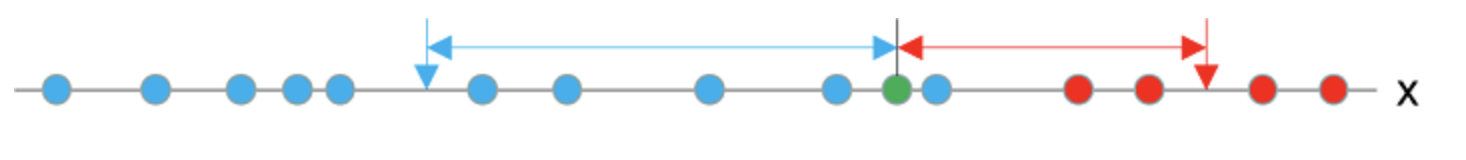
\includegraphics[width=14cm]{../pics/mahara.png}
  \caption{マハラノビスの汎距離}
  \label{fig:mahalanobis}
\end{figure}

式\eqref{eq:eq:Mahalanobis}を用いると, 式\eqref{eq:stat_unbiased_estimate}は次のようになる. 
\begin{align}
  \label{eq:stat_ve}
  t
  = \frac{Y_0-\eta_0}
  {\sqrt{\left\{
    \frac{1}{n} + \frac{1}{n}\operatorname{D}_0^2
  \right\}\operatorname{V}_e}}
\end{align}
このとき, $t$は自由度$n-p-1$のt分布に従い, $\eta_0$に対する信頼率$1-\alpha$の信頼区間は, 
\begin{align*}
  -t_{\alpha}(n-p-1) \leq
  \frac{Y_0-\eta_0}
  {\sqrt{\left(
    \frac{1}{n} + \frac{1}{n}\operatorname{D}_0^2
  \right)\operatorname{V}_e}}
  \leq t_{\alpha}(n-p-1)
\end{align*}
すなわち, 
\begin{align}
  \label{eq:confidence_interval}
  Y_0-t_{\alpha}(n-p-1)\sqrt{\left\{
    \frac{1}{n} + \frac{1}{n}\operatorname{D}_0^2
  \right\}}\operatorname{V}_e 
  \leq \eta_0
  \leq Y_0 + t_{\alpha}(n-p-1)\sqrt{\left\{
    \frac{1}{n} + \frac{1}{n}\operatorname{D}_0^2
  \right\}}\operatorname{V}_e 
\end{align}
のようになる. 式\eqref{eq:confidence_interval}で, $\operatorname{D}_0^2$の小さいところ, すなわち重心の近くでは信頼区間の巾が小さく, $\operatorname{D}_0^2$の大きいところ, すなわち重心から遠く離れたところでは信頼区間の巾が大きくなることがわかる.  \\

次に, 説明変数の特定の値$(x_{10}, \cdots, x_{p0})$に対応して得られるであろう目的変数$y$の値の信頼区間について考える. $y$は今までに観測されている$(y_1, \cdots, y_n)$やそれらに基づく$\hat{a}_1, \cdots, \hat{a}_p$とは独立に平均$\eta_0$, 分散$\sigma^2$の正規分布に従うため, $Y_0-y$の期待値と分散は, 
\begin{align}
  \notag
  \operatorname{E}(Y_0-y)
  &= \operatorname{E}(Y_0) - \operatorname{E}(y)\\
  \notag
  &= \eta_0 -\eta_0 \text{\quad ($\because$ 式\eqref{eq:eta_0} \;$\operatorname{E}(Y_0)=\eta_0$より)} \\
  \label{eq:E_y0-y}
  &= 0 \\
  \notag
  \\
  \notag
  \operatorname{V}(Y_0-y)
  &= \operatorname{E}\left[
    (Y_0-y)^2
  \right] \\
  \notag
  &= \operatorname{E}\left[
    \left\{
      (Y_0-\eta_0) - (y-\eta_0)
    \right\}^2
  \right] \\
  \notag
  &= \operatorname{E}\left[
    (Y_0-\eta_0)^2
  \right]
  +\operatorname{E}\left[
    (y-\eta_0)^2
  \right]
  -2\operatorname{E}\left[
    (Y_0-\eta_0)(y-\eta_0)
  \right] \\
  \notag
  &= \operatorname{V}(Y_0) + \operatorname{V}(y)-2\operatorname{Cov}(Y_0, y) \\
  \notag
  &=\operatorname{V}(Y_0) + \operatorname{V}(y) \text{\quad ($\because$ \;$Y_0$と$y$は無相関)} \\
  \notag
  &= \left(
    \frac{1}{n} + \frac{1}{n}\operatorname{D}_0^2
  \right)\sigma^2 
  + \sigma^2 \\
  \notag
  &\text{\quad ($\because$ 式\eqref{eq:v_y0} \;$\operatorname{V}(Y_0)=\left\{
    \frac{1}{n} + \frac{1}{n}\sum_{j=1}^p\sum_{l=1}^p(x_{j0}-\bar{x}_j)(x_{l0}-\bar{x}_l)s^{jl}
  \right\}\sigma^2$より)} \\
  \label{eq:V_y0-y}
  &= \left(
    1+\frac{1}{n} + \frac{1}{n}\operatorname{D}_0^2
  \right)\sigma^2
\end{align}
となる. これを用いて, $Y_0-y$を標準化し, $\sigma^2$を不偏推定値$\operatorname{V}_e=\frac{\operatorname{F}(\hat{a}_0, \hat{a}_1, \cdots, \hat{a}_p)}{n-p-1}$で置き換えると, 式\eqref{eq:t'}を得る. $t'$は自由度$n-p-1$のt分布に従う. 
\begin{align}
  \label{eq:t'}
  t'
  = \frac{Y_0-y}{\sqrt{\left(
    1+\frac{1}{n} + \frac{1}{n}\operatorname{D}_0^2
  \right)\operatorname{V}_e}}
\end{align}
これより, $(x_{10}, \cdots, x_{p0})$に対応して観測される目的変数$y$に対する信頼率$1-\alpha$の信頼区間は, 
\begin{align*}
  -t_\alpha(n-p-1) 
  \leq \frac{Y_0-y}{\sqrt{\left(
    1+\frac{1}{n} + \frac{1}{n}\operatorname{D}_0^2
  \right)\operatorname{V}_e}}
  \leq t_\alpha(n-p-1) 
\end{align*}
すなわち, 
\begin{align}
  \label{eq:confidence_interval_Y0}
  Y_0-t_{\alpha}(n-p-1)\sqrt{\left(
    1+\frac{1}{n} + \frac{1}{n}\operatorname{D}_0^2
  \right)\operatorname{V}_e}
  \leq y \leq
  Y_0+t_{\alpha}(n-p-1)\sqrt{\left(
    1+\frac{1}{n} + \frac{1}{n}\operatorname{D}_0^2
  \right)\operatorname{V}_e}
\end{align}
のように与えられる. 